In questa sezione sono riportate le implementazioni dei vari modelli utilizzati che si basano su due diverse tecniche per la generazione di word embeddings. Entrambe le tecniche conistono in metodi che vanno ad analizzare il testo creando degli embeddings, ovvero delle rappresentazioni compatte delle parole all'interno di uno spazio vettoriale dove due parole simili sono rappresentate da vettori simili. 

\subsection{GloVe}
In particolare la tecnica Global Vectors for Word Representation (GloVe) presentato in \cite{pennington2014glove} si basa sulla tecnica skip-gram e andandone a modificare la loss function introducendone alcune varianti per ridurne la complessità computazionale.
 \subsubsection{Skip-Gram with Global Corpus Statistics}
Si va a denotare con $q_{ij}$ la probabilità condizionata $P({w_{j}} | {w_{i}})$ di una parola contestuale $w_{j}$ data la parola target o centrale $w_{i}$ nel modello skip-gram:
\[q_{ij} = \frac{{\exp(\mathbf{u}_j \cdot \mathbf{v}_i)}}{{\sum_{k=1}^{V} \exp(\mathbf{u}_k \cdot \mathbf{v}_i)}}\]
La formula rappresenta la probabilità condizionata $q_{ij}$, che indica la probabilità che la parola di contesto $j$ si verifichi dato che la parola target $i$ è presente. Nella formula, $\mathbf{u}_j$ rappresenta il vettore di contesto per la parola di contesto $j$, $\mathbf{v}_i$ rappresenta il vettore della parola target $i$, e $\mathbf{u}_k$ rappresenta il vettore di contesto per qualsiasi altra parola $k$ nel corpus. La sommatoria nel denominatore si estende a tutte le parole nel vocabolario $V$ = \{0, 1, 2, \ldots, |V|-1\}.

La parola $w_{i}$ può presentarsi molte volte in un corpus. Tutte le parole contestuali che co-occorrono con wi creano un multiset, dove xij indica il conteggio del numero di volte che la parola wj co-occorre con wi nella stessa finestra di contesto nell'intero corpus. Utilizzando tali statistiche globali del corpus la loss function del modello skip-gram è:
\[-\sum_{i=1}^{V}\sum_{j=1}^{C} x_{ij} \log(q_{ij})\]
Inoltre, si denota con $x_{i}$ il numero delle parole di contesto dove compare $w_{i}$ come parola centrale. Si può definire come la probabilità condizionata $P_{ij} = \frac{x_{ij}}{x_i}$
di generare una parola di contesto $w_{j}$ data una parola centrale $w_{i}$ come:

\[-\sum_{i \in V} x_{i} \sum_{j \in V} p_{ij} \log q_{ij}\]

La sommatoria $-\sum_{j \in V} p_{ij} \log q_{ij}$ è la cross-entropy tra probabilità condizionata $q_{ij}$ relativa alla predizione generata dal modello, e $p_{ij}$ ottenuta analizzando le
statistiche dell'intero corpus.

\subsubsection{Modello GloVe}
Per ridurre la complessità computazionale (soprattutto per generare qij) e per mitigare gli effetti generati dai termini che compaiono di rado nel corpus ma che possono assumere importanza elevata dalla cross entropy, il modello GloVe introduce alcune varianti.


Il modello GloVe (Global Vectors for Word Representation) introduce alcune varianti al fine di ridurre la complessità computazionale e mitigare gli effetti dei termini rari nel corpus ma che potrebbero assumere importanza elevata dalla cross-entropy. I cambiamenti nella loss function consistono in:
\begin{itemize}
    \item Aggiunti due bias, $b_{i}$ per le parole centrali e $c_{i}$ per le parole contetsuali.  
    \item Utilizza delle nuove assegnazioni per evitare di utilizzare la probabilità condizionata $q_{ij}$ modificando la loss e introducendo gli ultimi due termini nel termine al quadrato.
    \item Si rimpiazza il peso di ogni termine della loss con una weight function $h_{x_{ij}}$ che varia nell'intervallo $[0,1]$.
\end{itemize}

Ottenendo come nuova loss function:
\[\sum_{i=1}^{V}\sum_{j=1}^{V} h(x_{ij}) \left( \mathbf{u}_j^T \mathbf{v}_i + b_i + c_j - \log x_{ij} \right)^2\]


  \subsubsection{GloVe - CNN1d}
  L'implementazione con le Convolutional Neural Networks (CNNs) impiega GloVe per generare gli embeddings, una serie di strati conv1D seguiti da GlobalMaxPooling1D e infine alcuni layer MLP con una softmax sull'ultimo strato dense con 3 nodi pari al numero di classi in output. Il dettaglio è indicato in Table \ref{tab:cnn}.

\begin{table}[!ht]
\centering
\caption{GloVe-CNN1d detailed model architecture}
\label{tab:cnn}
\begin{tabular}{ccccc}
\toprule
Layer & Maps & Kernel size & Activation & Dropout prob.\\
\midrule
    GloVe Embedding & - & - & - & - \\
    Convolution1d & 200 & 2x2 & ReLU & -\\
    GlobalMaxPooling1D & 200 & - & - & -\\
    Convolution1d & 200 & 3x3 & ReLU & -\\
    GlobalMaxPooling1D & 200 & - & - & -\\
    Convolution1d & 200 & 4x4 & ReLU & -\\
    GlobalMaxPooling1D & 200 & - & - & -\\
    Convolution1d & 200 & 5x5 & ReLU & -\\
    GlobalMaxPooling1D & 200 & - & - & -\\
    Convolution1d & 200 & 6x6 & ReLU & -\\
    GlobalMaxPooling1D & 200 & - & - & -\\
    Concatenate & 1000 & - & - & -\\
    Dropout & - & - & - & 0.1\\
    Fully Connected & 128 & - & ReLU & -\\
    Dropout & - & - & - & 0.2\\
    Fully Connected & 3 & - & Softmax & -\\
\bottomrule
\end{tabular}
\end{table}
\newpage

  \subsubsection{GloVe - LSTM}
  Anche l'implementazione con la Long short-term memory (LSTM) impiega GloVe per generare gli embeddings, successivamemte un layer ricorrente LSTM, un layer di flatten e infine alcuni layer MLP con una softmax sull'ultimo strato dense con 3 nodi pari al numero di classi in output. Nel dettaglio:
\begin{table}[!ht]
\centering
\caption{GloVe-LSTM detailed model architecture}
\begin{tabular}{cccc}
\toprule
Layer & Nodes & Return sequences & Activation \\
\midrule
    GloVe Embedding & - & - & - \\
    LSTM & 256 & True & TanH \\
    Flatten & - & - & - \\
    Fully Connected & 3 & - & Softmax\\
\bottomrule
\end{tabular}
\end{table}
  
\newpage

\subsection{BERT}
Il modello BERT proposto in \cite{devlin2019bert} per la generazione degli word embeddings combina due approcci differenti: 
\begin{itemize}
    \item \textit{Context-Indipendent}: data una parola, il vettore generato non dipenderà dal contesto attuale per cui termini polisemici o relazioni semantiche del linguaggio naturale saranno ignorate.
    \item \textit{Context-sensitive}: si combinano le rappresentazioni intermedie per ottenere una rappresentazione che dipende dalla sequenza in input.
\end{itemize}
BERT rappresenta l'intero contesto mediante un approccio bidirezionale e si basa su un architettura encoder-decoder di trasformers pre-addestrati su auxiliary task. Dell'intera architettura transformers verrà utilizzata però solamente l'encoder dato che l'obiettivo di questo modello è quello di generare un language model. 
In particolare in input c'è un singolo testo o una coppia di testi, che permette di andare a definire due auxiliary task differenti su cui è stata pre-addestrata la rete sui cui poi sarà possibile effettuare fine-tuning in base al contesto specifico. \newline
Un primo auxiliary task chiamato \textit{Next Sentence Prediction} consiste nel prendere coppie di testi e far predire alla rete se la seconda frase in coppia  è la frase successiva nel documento originale. Durante l'addestramento, il 50\% degli input è una coppia in cui la seconda frase è la frase successiva nel documento originale, mentre nell'altro 50\% viene scelta una frase random dal corpus come seconda frase. L'assunzione si basa sul fatto che la frase casuale sia slegata dalla prima frase.
\newline
Alla coppia di frasi si si aggiungono in fase di tokenizzazione due special token, rispettivamente \textit{CLS} inserito all'inizio della frase e \textit{SEP} inserito alla fine di ogni farse e poi successivamente viene sommato il sentence embedding che andrà a rappresentare se si la frase in questione è la frase A o la frase B. I due embedding così descritti verranno poi sommati ai positional embedding classici di un'architettura transformers, rappresentanti la posizione di un termine rispetto agli altri in una certa frase.\newline
Per andare poi a predire se la seconda frase è effettivamente collegata alla prima l'intera sequenza in input viene passata all'interno del modello e tramite uno strato di classificazione binaria insieme ad una softmax come funzione di attivazione si ottiene la predizione.
\newline
Dal modello pre-addestrato su questo auxiliary task appena descritto si è andato poi ad effettuare fine-tuning per il task obiettivo del progetto, ovvero la Sentiment Analysis.
Un ulteriore auxiliary task utile in altri contesti su cui gli autori di BERT hanno pre-addestrato il modello è il \textit{Masked Language Modeling}, dove dato un corpus testuale il 15\% dei tokens saranno selezionati in modo random per il task di predizione e al loro posto sarà presente un tag [mask].

\begin{figure}[!ht]
    \centering
    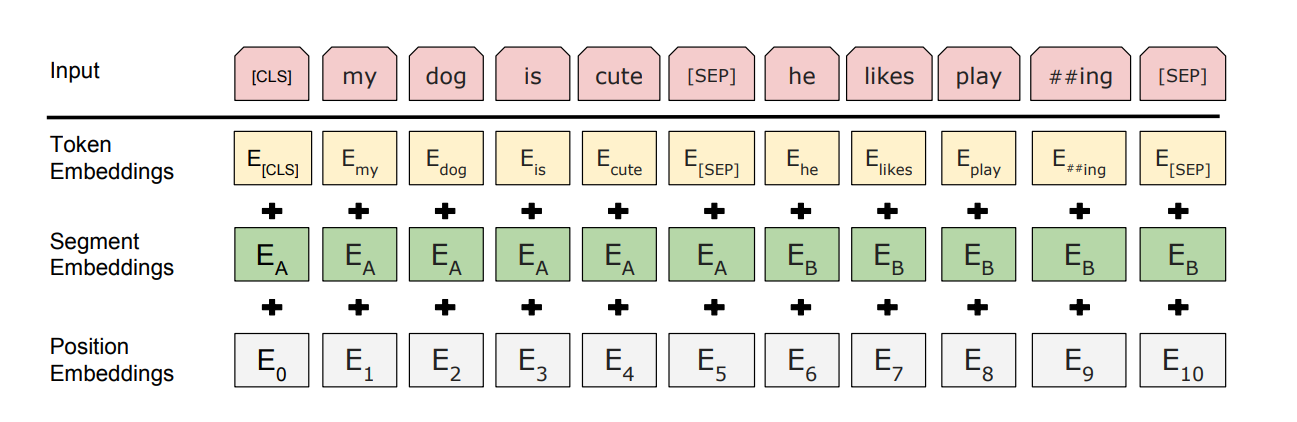
\includegraphics[width=15cm]{./images/bert.png}
    \caption{BERT input representation}
\end{figure}

\newpage
Nel seguito verranno riportate le versioni pretrained e le implementazioni utilizzate per il caso d'uso.\newline
Su entrambe le versioni di BERT l'implementazione della classe wrapper realizzata con Tensorflow è la seguente:
\begin{table}[!ht]
\centering
\caption{BERT Wrapper detailed model architecture}
\begin{tabular}{cccc}
\toprule
Layer & Maps & Dropout prob. & Activation \\
\midrule
    Pretrained BERT layer & - & - & - \\
    GlobalMaxPooling1D & 768 & - & - \\
    Fully Connected & 128 & - & ReLU\\
    Dropout & - & 0.1 & - \\
    Fully Connected & 32 & - & ReLU\\
    Fully Connected & 3 & - & Softmax\\
\bottomrule
\end{tabular}
\end{table}


\subsubsection{FinBERT}
FinBERT \cite{araci2019finbert} è una versione su cui è stato effettuato ulteriore pre-training della versione base di BERT. Gli autori di questa versione, FinBERT, hanno ulteriormente addestrato la rete su un corpus di dati finanziari per effettuare anche Sentiment Analysis, il dataset che hanno utilizzato gli autori è il Financial PhraseBank, lo stesso dataset utilizzato nella presente. 
Il modello pre-addestrato di FinBERT utilizzato nel training e nella valutazione del modello è quello offerto dalla libreria HuggingFace.\footnote{\href{https://huggingface.co/ProsusAI/finbert}{Pretrained HuggingFace FinBERT from ProsusAI}}  

    
\subsubsection{DistilBERT}
DistilBERT \cite{sanh2020distilbert} è una versione più piccola, veloce e leggera di BERT base. Ha il 40\% in meno di parametri rispetto a bert-base-uncased, funziona il 60\% più velocemente, preservando al contempo oltre il 95\% delle prestazioni di BERT misurate sul benchmark di comprensione del linguaggio GLUE. Il modello pre-addestrato di DistilBERT utilizzato nel training e nella valutazione del modello è stato sempre preso da HuggingFace.\footnote{\href{https://huggingface.co/distilbert-base-uncased}{Pretrained HuggingFace distilbert-base-uncased}}  



% https://towardsdatascience.com/bert-explained-state-of-the-art-language-model-for-nlp-f8b21a9b6270

% https://arxiv.org/pdf/1810.04805.pdf 